\documentclass{article}
\usepackage{iclr2027_conference,times}
\usepackage{hyperref}
\usepackage{url}
\usepackage{graphicx}
\usepackage{booktabs}
\usepackage{array}
\usepackage{amsmath,amssymb}
\usepackage{xcolor}
\usepackage{float}

% Independent rewrite built from the archived, versioned evidence.
% Submission mode remains off until the authors approve the final package.
\title{Auditing AI-Generated Harness Populations:\\
From One-Run Diversity to Stable Complementarity}
\author{Anonymous}

\newcommand{\bare}{\texttt{bare}}
\newcommand{\react}{\texttt{react}}
\newcommand{\pp}{\,pp}
% Generated by experiment.revision.render; post-review reanalysis.
\newcommand{\RevisionPrimaryDelta}{-0.16}
\newcommand{\RevisionPrimaryCI}{[-0.83,\ +0.87]}
\newcommand{\RevisionPrimaryP}{0.647}
\newcommand{\RevisionPrimaryRange}{-4.36\text{ to }+2.74}
\newcommand{\RevisionGateDelta}{-0.69}
\newcommand{\RevisionGateHolm}{0.079}
\newcommand{\RevisionOracleDelta}{-0.44}
\newcommand{\RevisionBestDelta}{-0.28}
\newcommand{\RevisionKmatchedDelta}{-0.31}
\newcommand{\RevisionKmatchedCI}{[-1.07,\ +0.40]}
\newcommand{\RevisionRtwoCached}{+0.42}
\newcommand{\RevisionRtwoOff}{+0.81}
\newcommand{\RevisionRtwoChange}{+0.39}
\newcommand{\RevisionRtwoChangeCI}{[-0.95,\ +1.63]}
\newcommand{\RevisionRtwoFlips}{2391}
\newcommand{\RevisionRtwoFlipPercent}{8.54}
\newcommand{\RevisionRtwoRepeatFlips}{1245}
\newcommand{\RevisionRtwoRepeatPercent}{8.65}
\newcommand{\RevisionRtwoLegacyCached}{-0.11}
\newcommand{\RevisionRtwoLegacyOff}{+0.36}
\newcommand{\RevisionCostRows}{153{,}600}
\newcommand{\RevisionLogicalCalls}{259{,}304}
\newcommand{\RevisionWoneOracle}{+0.35}
\newcommand{\RevisionWoneBest}{-0.42}
\newcommand{\RevisionWoneHeadroom}{+0.78}
\newcommand{\RevisionWoneFixed}{-0.001}
\newcommand{\RevisionWthreeSameSQL}{364{,}428}
\newcommand{\RevisionWthreeSameDisagreements}{0}
\newcommand{\RevisionWthreeRho}{0.597}
\newcommand{\RevisionWthreeWithinRho}{0.588}
\newcommand{\RevisionWthreeCallChanges}{506}
\newcommand{\RevisionWthreeSQLChanges}{19569}
\newcommand{\RevisionWthreeSQLN}{27936}
\newcommand{\RevisionWthreeSQLPercent}{70.05}
\newcommand{\RevisionWthreeJaccard}{0.619}

% Cross-domain mini-audit values; source-verified from artifacts/gsm8k_audit/metrics.json.
\newcommand{\RevisionMathHarnesses}{35}
\newcommand{\RevisionMathTasks}{400}
\newcommand{\RevisionMathDisagreement}{10.6}
\newcommand{\RevisionMathOracle}{98.50}
\newcommand{\RevisionMathBest}{93.75}
\newcommand{\RevisionMathHeadroom}{4.75}


\providecommand{\tightlist}{\setlength{\itemsep}{0pt}\setlength{\parskip}{0pt}}

\begin{document}
\maketitle

\begin{abstract}
An automatically generated harness can differ from its peers in source code,
execution trace, and correctness outcomes. These differences are often treated
as evidence of complementary capability, although each can also arise from an
inactive branch, an invalid implementation, or stochastic execution. We study
this measurement problem for harnesses wrapping a frozen language model on BIRD
text-to-SQL. A discovery population contained 36 outcome-identical pairs among
91 pairs despite source-code differences; trace audits separated absent,
untriggered, and broken mechanisms. We then reanalyze a frozen $2\times2$
study crossing strategy forcing with conformance gating over six builders and
three seeds. On 1,169 isolated questions, free ungated generation already had
8.56\pp bare-inclusive oracle headroom. The archived forced-and-gated versus
free-and-ungated contrast was $\RevisionPrimaryDelta\pp$ (95\% CI
$\RevisionPrimaryCI$), with no clear improvement. The gate also excludes two
allowed prompt-level strategies, so this is a combined screening and
conformance contrast rather than a pure verification effect. Repeated
executions further show that one-run oracle headroom can be created by the
same code. We therefore distinguish source diversity, executed mechanisms,
one-run outcome diversity, stable complementarity, and realized selection
utility. The current evidence motivates an auditable protocol for measuring
these quantities, but does not establish stable additional capability.
\end{abstract}

\section{Introduction}

Large language models are increasingly deployed inside harnesses: programs
that organize prompts, tool calls, state, verification, and output formatting
around a frozen model. Harness-generation systems can produce many candidate
programs, creating a natural population-selection problem. A common analysis
asks whether the candidates have different source code or whether their
correctness vectors differ on a test set. Neither observation answers the
practical question that matters for deployment:

\begin{quote}
Does the population contain additional capability that survives independent
executions and can be selected at a fixed cost?
\end{quote}

The distinction is easy to lose. A branch may be described but never executed;
a repair branch may exist but never be triggered; two valid mechanisms may
produce the same answer on the sampled tasks; or one stochastic execution of a
single harness may look like several complementary harnesses. In each case,
source-level diversity can overstate behavioral diversity, and one-run
behavioral diversity can overstate stable complementarity.

We examine these failure modes on BIRD text-to-SQL \citep{bird2021}. The paper
has two stages. Phase I is a discovery study that documents the measurement
problem in an early generated population. Phase II is a frozen factorial study
that asks whether strategy forcing and conformance gating change the observed
bare-inclusive oracle headroom under a common generation budget. We report a
post-review reanalysis of the archived Phase-II outcomes. This reanalysis
corrects the resampling and data-loading chain; it does not add independent
executions or repair the original gate.

Our contributions are deliberately narrower than a claim that generated
harnesses improve deployment performance:
\begin{enumerate}
\tightlist
\item We define separate measurements for source, trace, outcome, and stable
complementarity, and give a counterexample showing why oracle headroom is not
monotone in population size.
\item We provide a trace-based audit taxonomy and a factorial analysis that
makes the implemented admission policy explicit, including its structural
exclusion of two allowed prompt strategies.
\item We report the evidence boundary exposed by repeated execution,
fixed-$K$ sensitivity, and post-hoc selection analyses. These controls show
why a positive one-run headroom value is a necessary diagnostic for routing
research, but not evidence of a usable selector.
\end{enumerate}

The central unresolved test is a cost-matched comparison between a population
of genuinely different harnesses and a clone population formed by independent
executions of the same code. The present data do not contain that control; we
keep stable complementarity as an estimand rather than presenting it as a
finding.

\section{Related Work}

Recent work generates, evolves, or routes harnesses around frozen language
models, including harness evolution, self-harnessing, just-in-time harness
generation, and task--harness co-evolution \citep{tthe2026,selfharness2026,
jitagent2026,coevolve2026}. Concurrent behavior-aware systems use traces or
semantic screening inside their search loops \citep{harnesslens2026,
harnessfix2026,ahe2026,gatedqd2026,handbook2026}. Our question is different:
what properties does the resulting population have as an outcome matrix, and
which generation or admission policy changes those properties?

The distinction matters because a behavior-aware gate inside an evolution loop
does not by itself establish population complementarity. Likewise, portfolio
routing and algorithm-selection work assumes that candidate systems provide
reliable conditional value \citep{rice1976,xu2008satzilla,kotthoff2016}; our
study measures the conditions that a future router would need to inherit.
HELIX and related work emphasize sibling-harness outcome matrices and
complementarity \citep{helix2026}, while studies of harness sensitivity show
that no single harness need dominate across instances
\citep{nouniversal2026,nonmonotone2026}. We build on these ideas by separating
one-run coverage from repeat-stable value and by auditing the instrument that
decides whether a mechanism was actually present.

\section{Measurement Framework}

Let $H$ wrap a frozen target model $M$, receive an item $x$, make zero or more
model calls and tool executions, and return an answer scored by a judge. Let
$H_0$ be the bare single-call baseline and $Y(x,H,M)\in\{0,1\}$ its correctness.
The item-level marginal value is
\[
\Delta(x,H,M)=Y(x,H,M)-Y(x,H_0,M).
\]
For a population $P$, we report three one-run quantities. Pairwise outcome
disagreement is the fraction of items on which two members have different
correctness. Union repair is the fraction of bare errors repaired by at least
one member. Bare-inclusive oracle headroom is
\[
H(P)=\operatorname{Acc}\left(x\mapsto\max_{H\in P\cup\{H_0\}}Y(x,H,M)\right)
-\max_{H\in P\cup\{H_0\}}\operatorname{Acc}(H).
\]
Positive $H(P)$ means that, in this particular outcome matrix, different
members cover different items beyond the best fixed member. It does not imply
that a selector can identify those members before seeing the answer.

Headroom is not monotone in $|P|$. If two members solve complementary halves,
oracle accuracy can be 100\% and best-fixed accuracy 50\%. Adding a member that
solves every item leaves oracle accuracy at 100\% but raises best-fixed
accuracy to 100\%, reducing headroom to zero. Thus fixed-$K$ analyses are
sensitivity analyses, not proofs of a population-size mechanism.

For independent executions, let $p_{h,x}$ be the probability that harness $h$
solves item $x$. A repeat-stable analogue is
\[
H_{\mathrm{stable}}=\frac{1}{n}\sum_x\max_h p_{h,x}
-\max_h\frac{1}{n}\sum_xp_{h,x}.
\]
A clone population whose members are the same code has identical $p_{h,x}$
and therefore zero stable headroom, even though separate one-run executions
can produce positive oracle headroom. Estimating this quantity requires
independent repeats and a selector evaluation that is separated from the
observations used to fit it.

\section{Phase I: Discovery Audit}

Phase I uses GLM-5.3-Flash at temperature zero on 60 BIRD questions. It is
discovery evidence: 24 items overlapped protocol development, the human
positive control was designed after trace inspection, and the legacy judge was
a conservative proxy. These conditions support diagnosis, not confirmation.

The day-1 population contains \bare{}, \react{}, and 12 generated candidates.
Across all 14 harnesses, 36 of 91 pairs have identical correctness vectors and
mean pairwise disagreement is 3.3\%. Among the 12 generated candidates alone,
21 of 66 pairs are identical and mean disagreement is 3.8\%. The candidate
pair code-similarity mean is 0.143 under the original normalized-character
metric. In the full population, the token-sequence metric used in Figure~\ref{fig:phenomenon}
has mean 0.190 and Spearman $\rho=-0.010$ with outcome disagreement. Pairs
share harnesses, so this is a descriptive summary rather than an independent
sample test.

\begin{figure}[H]
\centering
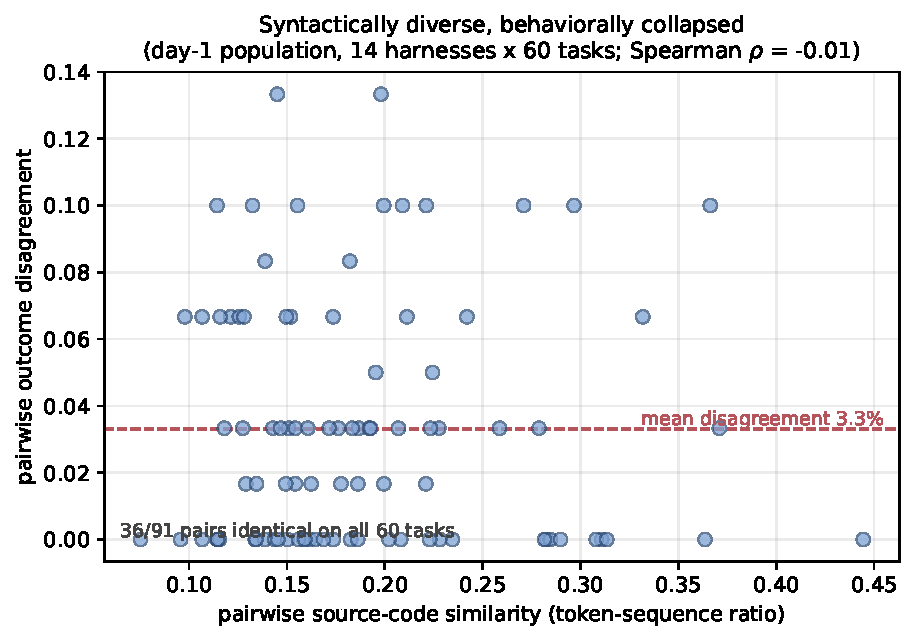
\includegraphics[width=0.62\linewidth]{figures/fig_phenomenon.pdf}
\caption{Phase-I discovery audit. Each point is a pair among 14 harnesses on
60 tasks. Source-code similarity and outcome disagreement are distinct
measurements; $\rho=-0.01$ is descriptive, and 36/91 pairs are outcome
identical.}
\label{fig:phenomenon}
\end{figure}

Trace inspection identifies three actionable classes. T1 mechanisms are
described but absent from control flow: six of 12 candidates make one model
call and execute no artifact. T2 mechanisms are present but untriggered: in
all 10 audited \react{} tasks, the first SQL succeeds, so conditional repair
does not run. T3 is a broken multi-turn path: one candidate returns prose as
final SQL and turns some bare-correct items into errors. These classes require
different controls. A mechanism gate must test execution, a repair claim must
be tested with controlled faults, and a multi-turn harness must validate its
executable output.

Hand-written positive controls show that task-side headroom exists in the
observed matrix: forcibly distinct execution paths give 6.67\pp on 60 items
and 7.28\pp on a 151-item probe. Because the control was designed after
inspection, these values establish available headroom, not an unbiased effect
estimate.

\section{Phase II: Frozen Factorial Study}

Phase II crosses two factors over six builders and three seeds. The free arm
allows the builder to invent a mechanism; the forced arm assigns one of eight
named strategies. The ungated arm applies neutral validity checks; the gated
arm additionally requires the frozen conformance suite. We call the four arms
II-A (free/ungated), II-B (free/gated), II-C (forced/ungated), and II-D
(forced/gated). An open-mechanism arm II-E is secondary and outside the
factorial.

The conformance suite drives scripted scenarios and checks recorded traces,
including paired counterfactuals whose correct answers differ. It was calibrated
before Phase-II generation with three positive controls and two negative
impostors. The implemented gate maps both \texttt{hint\_guard} and
\texttt{format\_guard} to a no-mechanism result. Therefore II-D versus II-A
combines strategy forcing, structural screening, and conformance verification;
it cannot identify verification alone.

Each slot permits at most three raw builder attempts and stops at the first
accepted candidate. Realized attempts were 269, 255, 273, and 324 for II-A
through II-D against a 432-attempt arm cap; realized token cost is not fully
recovered. Slots are not topped up after failure, so generation reliability is
part of the policy and is reported separately from population quality.

The target is GLM-5.3-Flash. The primary set has 1,169 questions from nine
databases never opened during development, with a disclosed 18-item smoke-test
exception. All 18 builder--seed cells enter the primary analysis, including
empty populations. The official BIRD execution scorer is primary; the legacy
judge is a conservative secondary check. A 400-item core, frozen before
outcomes, supports the four-arm secondary analysis.

\begin{figure}[H]
\centering
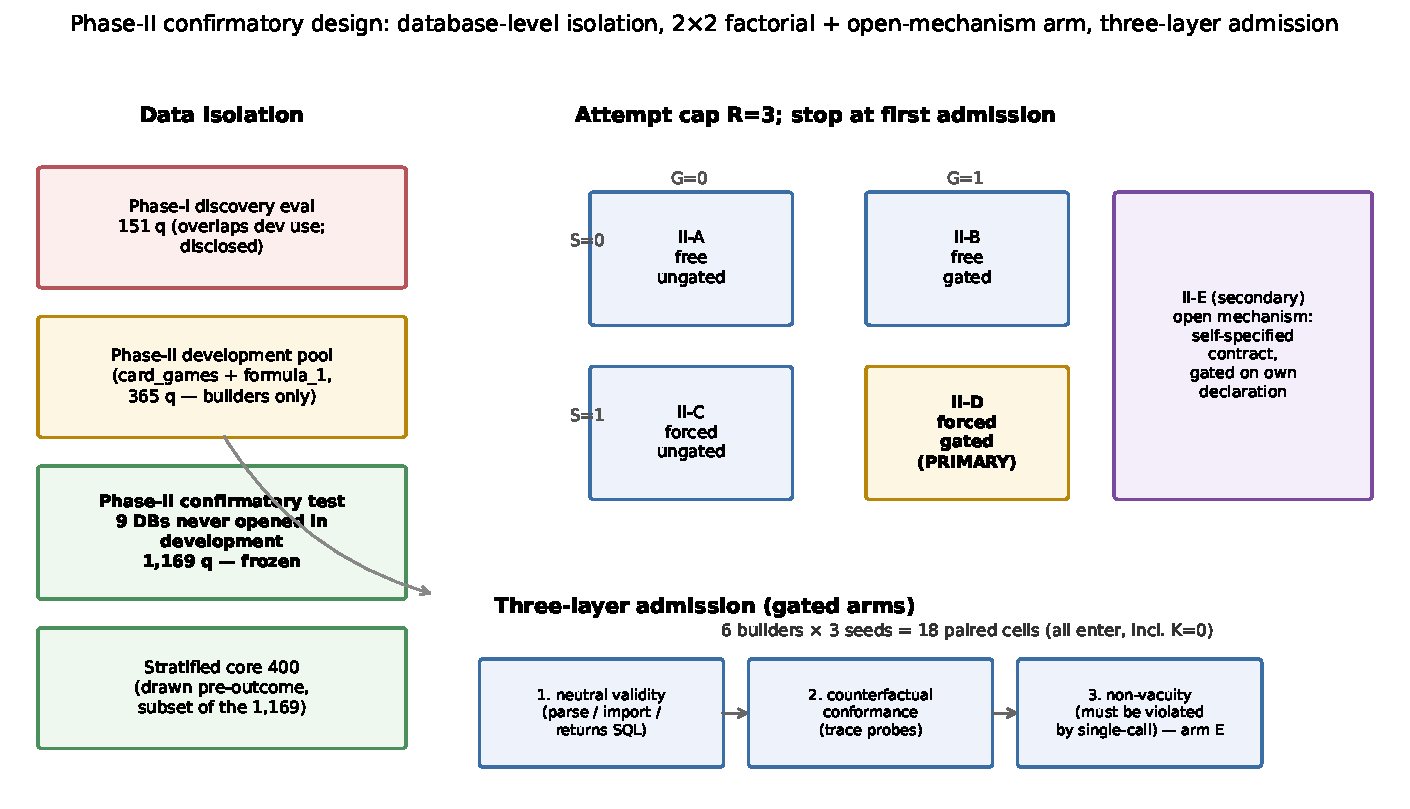
\includegraphics[width=0.58\linewidth]{figures/fig_design_revision.pdf}
\caption{Frozen Phase-II design. Strategy forcing and conformance gating are
crossed under a common raw-attempt cap; realized costs and admitted population
sizes can differ. The gate is a trace instrument with neutral validity,
counterfactual conformance, and non-vacuity checks.}
\label{fig:design}
\end{figure}

The primary estimand is the paired cell difference
$H(\mathrm{II\text{-}D})-H(\mathrm{II\text{-}A})$ on the full set. We use shared
database and within-database task resampling, generation-seed resampling within
builder, and a sign-flip reference test conditional on observed tasks. The
factorial secondary estimands on the common core are the gate main effect,
strategy main effect, and their interaction. These are conditional analyses of
archived executions, not randomized tests of an abstract gate.

\section{Results}

\subsection{Primary contrast}

Table~\ref{tab:primary} reports the corrected reanalysis. Free ungated
generation already produces 76.14\% oracle accuracy, 67.58\% best-fixed
accuracy, and 8.56\pp headroom. Forced gated generation produces 75.70\%
oracle accuracy, 67.30\% best-fixed accuracy, and 8.40\pp headroom. The paired
headroom contrast is $\RevisionPrimaryDelta\pp$ with 95\% CI
$\RevisionPrimaryCI$ and one-sided sign-flip $p=\RevisionPrimaryP$; cell
contrasts range from $\RevisionPrimaryRange\pp$.

\begin{table}[H]
\centering\small
\begin{tabular}{@{}lrr@{}}
\toprule
Metric & II-A & II-D \\
\midrule
Candidate count & 5.78 & 3.83 \\
Oracle accuracy (\%) & 76.14 & 75.70 \\
Best-fixed accuracy (\%) & 67.58 & 67.30 \\
Headroom (pp) & 8.56 & 8.40 \\
\midrule
D$-$A headroom (pp) & \multicolumn{2}{c}{$\RevisionPrimaryDelta$} \\
Unadjusted bootstrap 95\% CI & \multicolumn{2}{c}{$\RevisionPrimaryCI$} \\
One-sided sign-flip $p$ & \multicolumn{2}{c}{$\RevisionPrimaryP$} \\
\bottomrule
\end{tabular}

\caption{Corrected primary analysis of the archived intervention. Bare is
retained in oracle and best-fixed calculations. The interval reflects the
versioned task and generation-seed resampling chain, conditional on the six
builders and archived execution records.}
\label{tab:primary}
\end{table}

The interval does not establish equivalence, but it provides no clear evidence
that the implemented forced-and-gated policy improves headroom. Because the
gate excludes allowed prompt transformations, the result should not be
described as a pure conformance effect.

\subsection{Factorial and fixed-population sensitivity}

On the common 400-item core, the corrected gate main effect is -0.69\pp with
Holm-adjusted $p=0.079$; the strategy effect is +0.42\pp (adjusted $p=0.428$)
and the interaction is -0.87\pp (adjusted $p=0.428$). The fixed-$K$ gate
sensitivity is -0.31\pp with 95\% CI $[-1.07,+0.40]$. The reduction in a
subsampled contrast is a sensitivity result; it is not a causal decomposition
of how much population size mediated the original contrast.

\begin{table}[H]
\centering\small
\begin{tabular}{@{}lrrrr@{}}
\toprule
Contrast & Effect (pp) & 95\% CI (pp) & Raw $p$ & Holm $p$ \\
\midrule
Gate & $-0.69$ & $[-1.56, +0.20]$ & 0.026 & 0.079 \\
Strategy & $+0.42$ & $[-0.32, +1.51]$ & 0.263 & 0.428 \\
Interaction & $-0.87$ & $[-2.83, +0.65]$ & 0.214 & 0.428 \\
\bottomrule
\end{tabular}

\caption{Corrected factorial reanalysis on the common core. Gate, strategy,
and interaction estimands are defined by the four arm means. Raw tests use
cell sign flips and Holm correction covers the three secondary contrasts.}
\label{tab:factorial}
\end{table}

For the full primary set, oracle accuracy changes by -0.44\pp and best-fixed
accuracy by -0.28\pp from II-A to II-D. The difference in these components is
reported explicitly because headroom is an arithmetic diagnostic, not a
direct measurement of realized routing utility. Candidate counts also differ:
$K_{\rm cand}$ excludes bare and $K_{\rm total}=K_{\rm cand}+1$.

\begin{table}[H]
\centering\footnotesize
\begin{tabular}{@{}lrrrrrr@{}}
\toprule
Arm & $K_{\rm cand}$ & $K_{\rm total}$ & Single-call (\%) & Best (\%) & Oracle (\%) & $H$ (\%) \\
\midrule
A & 5.78 & 6.78 & 63.25 & 66.00 & 74.51 & 8.51 \\
B & 6.11 & 7.11 & 63.25 & 66.12 & 74.39 & 8.26 \\
C & 5.61 & 6.61 & 63.25 & 65.64 & 75.01 & 9.38 \\
D & 3.83 & 4.83 & 63.25 & 65.65 & 73.90 & 8.25 \\
\bottomrule
\end{tabular}

\caption{Same-core decomposition. All arms share the same bare outcomes.
Headroom is oracle accuracy minus best-fixed accuracy; it is not selector
accuracy.}
\label{tab:decomp}
\end{table}

\subsection{Execution variability and selection boundary}

Across three cache-off repeats, 14.5\% of bare tasks changed correctness at
least once. A canonical R2 replay found 2,391 same-harness verdict flips among
28,000 comparisons (8.54\%). The cache-off subset contrast changed from
$\RevisionRtwoCached\pp$ to $\RevisionRtwoOff\pp$; its change was
$\RevisionRtwoChange\pp$ with 95\% CI $\RevisionRtwoChangeCI$. These are
instability measurements, not standard errors or a noise floor for the primary
effect. They do not show that every contrast is unchanged.

As a direct diagnostic, three executions of the identical bare source treated
as if they were three population members yield 72.25\% one-run oracle accuracy
and 65.75\% best-fixed accuracy, a 6.50\pp artificial headroom gap on the same
400 tasks. The source hash is identical, so this result demonstrates only that
execution sampling can create one-run headroom.

The Phase-I leave-one-harness-out predictor did not beat the best fixed member
in the tested DeepSeek population (-3.4\pp); the Qwen estimate was +0.9\pp with
CI $[-5.2,+6.9]$. Database-stratified task-held-out controls reduced repair
AUROC to 0.512. A post-hoc diversity-selection analysis at $k=8$ changes
headroom by $\RevisionWoneHeadroom\pp$, with oracle accuracy changing by
$\RevisionWoneOracle\pp$ and best-fixed accuracy by $\RevisionWoneBest\pp$.
These analyses are descriptive and single-execution; they do not establish a
deployable router or practical selection gain.

\section{Discussion}

The results support a measurement conclusion. Code differences, executed
mechanisms, one-run correctness differences, repeat-stable complementarity,
and realized selector value are different objects. The Phase-I population makes
the first boundary visible. The Phase-II archive tests one policy contrast but
does not remove the second boundary: observed oracle headroom can contain
execution randomness, and the gate's structural exclusions prevent a pure
verification interpretation.

This framing also changes how population size should be interpreted. Increasing
the number of candidates can increase oracle coverage, leave it unchanged, or
reduce headroom if a strong fixed member improves the best-fixed comparator.
Similarly, a K-matched difference tells us how the estimand changes after
subsampling; it does not identify a causal share attributable to population
size.

The most informative next experiment is a cost-matched clone control. It should
use the same raw pool, interleave real and clone executions, run each code path
under cache-on and cache-off conditions, and reserve independent repeats for
validation. It should report absolute oracle accuracy, best-fixed accuracy,
realized selector accuracy if a selector is specified, candidate count, and
cost. A gate calibration set should separately include legal single-call
rewrites, conditional repair, unconditional extra calls, discarded feedback,
position-based voting, and untriggered repair. This is necessary to distinguish
an absent mechanism, an untriggered mechanism, a nonresponsive mechanism, and
an implementation failure.

The evidence is limited to one main target, six fixed builders, and three
generation seeds. Phase I contains development overlap and a post-trace human
control. The corrected analysis is post-review and does not add executions.
The one-seed MATH-500 probe in the supplement extends the outcome comparison to
a second domain, but has no clone control, repaired-gate factorial, or
independent stable-complementarity test. Partial provider acquisitions are
retained for provenance and missingness accounting and are excluded from
population-performance claims.

\section{Conclusion}

AI-generated harness populations should be audited at the level of what they
execute and what remains reliable across repeats. In our archived BIRD study,
the implemented forced-and-gated policy does not show a clear headroom gain,
and the available one-run headroom is not sufficient to claim stable
complementarity. The practical contribution is an evidence boundary: a
population becomes a candidate for reliable routing only after it passes
mechanism calibration, cost matching, repeat validation, and independent
selection evaluation.

\subsection*{AI use statement}
This work studies AI-generated artifacts and also used generative AI tools for
experimental code, model-call workflows, data analysis, figures, and
manuscript drafting. The archived tables and result values in this rewrite are
read from the versioned reanalysis artifacts; historical exploratory results
retain their stated provenance. AI tools also assisted with research design and
revision. The authors are responsible for the final scientific decisions,
claims, and submission.

\bibliography{references}
\bibliographystyle{iclr2027_conference}

\appendix
\section{Reproducibility Notes}

All main tables in this rewrite use the shared versioned macros and table
artifacts in the paper directory. The archived analysis distinguishes source
hash, task, repeat, cache condition, arm, membership, source file, and conflict
policy. Reproduction should begin from the canonical input order and should
report missing, duplicate, and conflicting records before computing aggregate
metrics. The full protocol changelog, gate controls, extraction audit,
cross-domain probe, and W1 sensitivity analysis remain in the existing
supplementary source files and must be synchronized before submission.

\end{document}
